
%
% File sem_syn_diff.tex

\documentclass[11pt,a4paper]{article}
\usepackage[hyperref]{emnlp2018}
\usepackage{times}
\usepackage{latexsym}
\usepackage{amsmath}
\usepackage{tikz}
\usepackage{tikz-dependency}
\usepackage[warn]{textcomp}
\usepackage[font=small]{caption}
\usepackage{subcaption}
\usepackage{multirow}
\usepackage{url}
\usepackage{etoolbox}
\usepackage{xr}
\usepackage{listings}

\newcommand{\com}[1]{}
\newcommand{\oa}[1]{\footnote{\color{red}OA: #1}}
\newcommand{\daniel}[1]{\footnote{\color{blue}Daniel: #1}}

\hyphenation{SemEval}

\DeclareMathOperator*{\argmin}{argmin}
\DeclareMathOperator*{\argmax}{argmax}

\lstset{basicstyle=\ttfamily}

\makeatletter
\patchcmd\@combinedblfloats{\box\@outputbox}{\unvbox\@outputbox}{}{%
   \errmessage{\noexpand\@combinedblfloats could not be patched}%
}%
 \makeatother


\usetikzlibrary{shapes,shapes.misc}

%\aclfinalcopy % Uncomment this line for the final submission
\def\aclpaperid{***}

%\setlength\titlebox{5cm}
% You can expand the titlebox if you need extra space
% to show all the authors. Please do not make the titlebox
% smaller than 5cm (the original size); we will check this
% in the camera-ready version and ask you to change it back.

\title{Why Semantics is Harder than Syntax}

\author{Daniel Hershcovich$^{1,2}$ \\
  \\\And
  Omri Abend$^2$ \\
  $^1$The Edmond and Lily Safra Center for Brain Sciences \\
  $^2$School of Computer Science and Engineering \\
  Hebrew University of Jerusalem \\
  \texttt{\{danielh,oabend,arir\}@cs.huji.ac.il}
  \\\And
  Ari Rappoport$^2$
}

\date{}

\begin{document}

\maketitle

\begin{abstract}
To explain the difference in scores between syntactic and semantic parsers,
we explore the various factors and perform experiments to demonstrate them.
As a test case, we take Universal Dependencies (UD) and
Universal Conceptual Cognitive Annotation (UCCA).
By creating a full conversion protocol, we develop a novel UCCA parser.
\end{abstract}

\section{Introduction}\label{sec:introduction}

Semantic representation schemes have seen major progress in recent years.
In parallel, syntactic representation is becoming more semantic.
However, looking at the absolute scores achieved in semantic parsing tasks
as opposed to syntactic parsing,
there is still a gap:
UCCA parsers get just about 75\% F-score, whereas UD parsers get more than 85\% LAS F1. Why?
UD has much more training data (UCCA: 5K, UD: about 17K for English).
But inter-annotator agreement is also lower: about 85\% for UCCA, and more than 95\% for UD.

Several questions naturally manifest themselves:
how much of the difference is explained by the differences in---
\begin{itemize}
\item Evaluation metric,
\item Amount of training data,
\item Content.
\end{itemize}

The gap can be explained by fine-grained semantic annotation such as adposition and case supersenses
\cite{schneider2017adposition,blodgett2018semantic}.

To explore the difference in content, we experiment with converting UD to UCCA
using a multi-step protocol:
\begin{enumerate}
\item Augment UD trees to get \textit{enhanced++} dependencies \cite{SCHUSTER16.779}, hence UD$^{++}$.
\item Structurally convert bilexical dependency graphs into constituency-like graphs by inserting
  non-terminal nodes and \textit{head} edges (\S\ref{sec:conversion}).
\item Translate UD relations into UCCA edge labels,
  either by a deterministic mapping (\S\ref{sec:mapping})
  or through learning (\S\ref{sec:learning}).
\end{enumerate}

%%%%%%%%%%%%%%%%%%%%%%%%%%%%%%%%%%%%%%%%%%%%%%%%%%%%%%%%%%%%%%%%%%%%%%%%%%%%%%%%%
\section{Related Work}\label{sec:related_work}

\paragraph{AMR parsing.}

\citet{wang2015transition,wang-xue-pradhan:2015:ACL-IJCNLP,wang-EtAl:2016:SemEval,goodman2016noise,wang2017getting}
presented a transition-based AMR parser, CAMR, which requires a
syntactic dependency tree as input.
It operates on the input tree, transforming it into an AMR graph
by a sequence of transitions.
The accuracy of the underlying syntactic dependency parser is important,
as shown by \citet{wang-xue-pradhan:2015:ACL-IJCNLP},
who achieved the best results using the Charniak parser trained on a
much larger and more diverse dataset---the full OntoNotes corpus,
rather than the Stanford parser trained on the Penn TreeBank.


%%%%%%%%%%%%%%%%%%%%%%%%%%%%%%%%%%%%%%%%%%%%%%%%%%%%%%%%%%%%%%%%%%%%%%%%%%%%%%%%%

\section{Representations}\label{sec:representations}

\paragraph{Universal Conceptual Cognitive Annotation.}\label{sec:ucca}
UCCA \cite{abend2013universal} is a semantic representation whose main design principles
are ease of annotation, cross-linguistic applicability, and a modular architecture.
UCCA represents the semantics of linguistic utterances
as directed acyclic graphs (DAGs), where terminal (childless) nodes
correspond to the text tokens, and non-terminal nodes to semantic units that participate
in some super-ordinate relation.
Edges are labeled, indicating the role of a child in the relation the parent represents.
Nodes and edges belong to one of several \textit{layers}, each corresponding
to a ``module'' of semantic distinctions.
UCCA's \textit{foundational layer} (the only layer for which annotated data exists)
mostly covers predicate-argument structure, semantic heads and inter-Scene relations.

UCCA distinguishes \textit{primary} edges, corresponding 
to explicit relations, from \textit{remote} edges (appear dashed in
Figure~\ref{fig:example_ucca}) that allow for a unit to participate
in several super-ordinate relations.
Primary edges form a tree in each layer, whereas remote edges enable reentrancy, forming a DAG.


\begin{figure}[!ht]
  \centering
    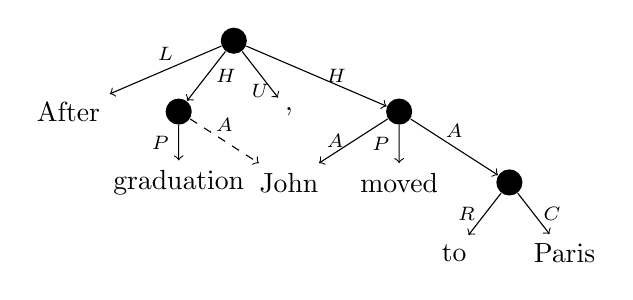
\begin{tikzpicture}[level distance=9mm, sibling distance=14mm, ->,
        every circle node/.append style={fill=black}]
      \tikzstyle{word} = [font=\rmfamily,color=black]
      \node (ROOT) [circle] {}
        child {node (After) [word] {After} edge from parent node[above] {\scriptsize $L$}}
        child {node (graduation) [circle] {}
        {
          child {node [word] {graduation} edge from parent node[left] {\scriptsize $P$}}
        } edge from parent node[right] {\scriptsize $H$} }
        child {node [word] {,} edge from parent node[below] {\scriptsize $U$}}
        child {node (moved) [circle] {}
        {
          child {node (John) [word] {John} edge from parent node[left] {\scriptsize $A$}}
          child {node [word] {moved} edge from parent node[left] {\scriptsize $P$}}
          child {node [circle] {}
          {
            child {node [word] {to} edge from parent node[left] {\scriptsize $R$}}
            child {node [word] {Paris} edge from parent node[right] {\scriptsize $C$}}
          } edge from parent node[above] {\scriptsize $A$} }
        } edge from parent node[right] {\scriptsize $H$} }
        ;
      \draw[dashed,->] (graduation) to node [above] {\scriptsize $A$} (John);
    \end{tikzpicture}
\caption{\label{fig:example_ucca}
 Example UCCA graph. The dashed edge is remote.
  Pre-terminal nodes and edges are omitted for brevity.}
\end{figure}

%%%%%%%%%%%%%%%%%%%%%%%%%%%%%%%%%%%%%%%%%%%%%%%%%%%%%%%%%%%%%%%%
\paragraph{Universal Dependencies.}\label{sec:ud}
UD \cite{nivre2016universal,11234/1-2515} has quickly become
the dominant dependency scheme for
syntactic  annotation in many languages,
aiming for cross-linguistically consistent and coarse-grained treebank
annotation. Formally, UD uses bilexical trees, with edge labels 
representing syntactic relations between words.
Figure~\ref{fig:original_example_ud} shows an example UD tree.

We use UD as an auxiliary task,
inspired by previous work on joint syntactic and semantic parsing
(see \S\ref{sec:related_work}).
In order to reach comparable analyses cross-linguistically,
UD often ends up in annotation that is similar to the common practice
in semantic treebanks, such as linking content words to content words wherever possible.
Using UD further allows conducting experiments on languages other than English, 
for which AMR and SDP annotated data is not available (\S\ref{sec:experiments}).

In addition to basic UD trees, we use the \textit{enhanced++} UD graphs available for English,
which are generated by the Stanford CoreNLP converters \cite{SCHUSTER16.779}.
These include additional and augmented relations between content words,
partially overlapping with the notion of remote edges in UCCA:
in the case of control verbs, for example, a direct relation is added in 
enhanced++ UD between the subordinated verb and its controller,
which is similar to the semantic schemes' treatment of this construction.

\begin{figure}[!ht]

\fbox{\begin{subfigure}{0.47\textwidth}
  \centering
    \begin{dependency}[text only label, label style={above}, font=\small]
    \begin{deptext}[column sep=.8em,ampersand replacement=\^]
    After \^ graduation \^ , \^ John \^ moved \^ to \^ Paris \\
    \end{deptext}
        \depedge[edge unit distance=1ex]{2}{1}{case}
        \depedge[edge unit distance=1ex]{4}{3}{punct}
        \depedge[edge unit distance=1ex]{5}{4}{nsubj}
        \depedge[edge unit distance=1ex, edge end x offset=-2pt]{2}{5}{obl}
        \depedge[edge unit distance=1ex]{7}{6}{case}
        \deproot[edge unit distance=1.5ex]{5}{root}
        \depedge[edge unit distance=1.5ex]{5}{7}{obl}
    \end{dependency}
  \caption{UD \label{fig:original_example_ud}}
\end{subfigure}}

\fbox{\begin{subfigure}{0.47\textwidth}
  \centering
  \scalebox{.95}{
  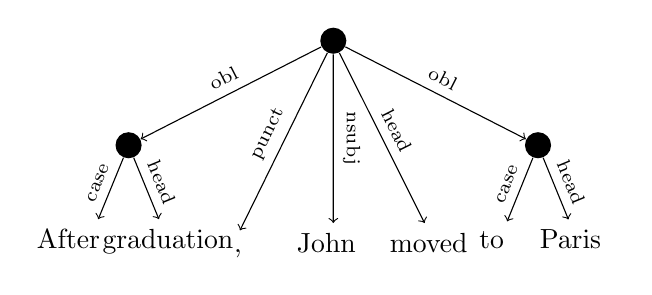
\begin{tikzpicture}[level distance=15mm, ->,
      every node/.append style={sloped,anchor=south,auto=false,font=\scriptsize},
      level 1/.style={sibling distance=13mm},
      level 2/.style={sibling distance=1cm}]
    \tikzstyle{word} = [font=\rmfamily,color=black]
    \node (ROOT) [fill=black,circle] {}
      child {node (after) [fill=black,circle] {}
      {
        child {node [word] {After{\color{white}g}\quad\quad} edge from parent node {case}}
        child {node [word] {\quad graduation\quad\quad} edge from parent node {head}}
      } edge from parent node {obl}}
      child {node {}
      {
        child {node [word] (comma) {\quad,{\color{white}g}} edge from parent [draw=none]}
      } edge from parent [draw=none]}
      child {node {}
      {
        child {node [word] (John) {John{\color{white}g}} edge from parent [draw=none]}
      } edge from parent [draw=none]}
      child {node {}
      {
        child {node [word] (moved) {moved{\color{white}g}} edge from parent [draw=none]}
      } edge from parent [draw=none]}
      child {node (to) [fill=black,circle] {}
      {
          child {node [word] {to{\color{white}g}} edge from parent node {case}}
          child {node [word] {Paris{\color{white}g}} edge from parent node {head}}
      } edge from parent node {obl}}
      ;
      \draw (ROOT) to node {punct} (comma);
      \draw (ROOT) to node {nsubj} (John);
      \draw (ROOT) to node {head} (moved);
  \end{tikzpicture}}
  \captionof{figure}{UD}\label{fig:converted_example_ud}
\end{subfigure}}

\caption{Figure \ref{fig:original_example_ud} presents a UD tree.
  Edge labels express syntactic relations.
Figure~\ref{fig:converted_example_ud} presents a converted UD graph
(with pre-terminals omitted: each terminal drawn in place of its parent).
Intermediate non-terminals and \textit{head} edges are introduced.
While converted UD graphs form trees, enhanced++ UD graphs may not.}\label{fig:ud_examples}
\end{figure}


\section{Amount of training data}\label{sec:data_size}

Syntactic dependency parsers require many training examples to achieve
state-of-the-art results.
Even after around 500K tokens, the learning curves do not seem to saturate
\cite{de2017old,velldal2017joint}.


\section{Structural Conversion}\label{sec:conversion}

We convert UD into a unified DAG format \cite{hershcovich2018multitask},
which is inclusive enough to
allow representing any of the schemes with very little loss of information.
For UD, and conversion results in 98.5\% LAS $F_1$ on the UD English test set,
due to multi-word tokens, not supported in the unified DAG format.

The format consists of a rooted DAG, where the tokens are the terminal nodes.
As in the UCCA format, edges are labeled (but not nodes),
and are divided into \textit{primary} and \textit{remote} edges,
where the primary edges form a tree (all nodes have at most one primary parent,
and the root has none).
Remote edges enable reentrancy, and thus together with primary edges
form a DAG.
Figure~\ref{fig:converted_example_ud} shows an example for a converted graph.

To convert UD into the unified DAG format,
we add a pre-terminal for each token,
and attach the pre-terminals according to the original dependency edges:
traversing the tree from the root down, for each head token we create a non-terminal
parent with the edge label {\it head},
and add the node's dependents as children of the created non-terminal node.
In case of reentrancy, an arbitrary parent is marked as primary, and the rest as remote
(denoted as dashed edges in Figure~\ref{fig:converted_example_ud}).

Table~\ref{tab:conversion_results_unlabeled} shows unlabeled evaluation of the
structurally converted UD graphs as compared to gold-annotated UCCA graphs.


\begin{table}[t]
\centering
\begin{tabular}{l|lll|lll}
& \multicolumn{3}{c|}{\footnotesize \bf Primary} & \multicolumn{3}{c}{\footnotesize \bf Remote} \\
& \footnotesize \textbf{UP} & \footnotesize \textbf{UR} & \footnotesize \textbf{UF}
& \footnotesize \textbf{UP} & \footnotesize \textbf{UR} & \footnotesize \textbf{UF} \\
\hline
\multicolumn{4}{l|}{\small \bf WSJ (manually annotated)} & \\
\footnotesize UD$^{++}$
& 84.6 & 85.6 & 85.1 & 12.5 & 12.7 & 12.6 \\
\end{tabular}
\caption{
Unlabeled precision, recall and $F_1$ (in~\%) for primary and remote edges.}\label{tab:conversion_results_unlabeled}
\end{table}


\section{Deterministic label mapping}\label{sec:mapping}


Using the standard UCCA evaluation
script,\footnote{\url{http://github.com/danielhers/ucca/blob/master/scripts/evaluate_standard.py}}
we created a confusion matrix between the edge tags in converted UD$^{++}$ graphs
\cite{SCHUSTER16.779}
and the annotated UCCA graphs (see Table~\ref{tab:confusion_matrix}).
Edges are matched by terminal yield.
In this confusion matrix, we can see what is the most common UCCA edge label corresponding
to each UD relation.
To convert the UD$^{++}$ graphs into fully labeled UCCA graphs,
we replace each UD edge label with its most common UCCA counterpart.

\begin{table}[t]
\centering
\begin{tabular}{ll|r}
UD & UCCA & count \\
\hline
head & C & 508 \\
case & R & 231 \\
det & E & 196 \\ 
amod & E & 129 \\
compound & E & 113 \\
head & P & 109 \\
nsubj & A & 106 \\
dobj & A & 51 \\
nummod & E & 33 \\
cc & N & 32 \\
advmod & D & 31 \\
conj:and & C & 26
\end{tabular}
\caption{Excerpt from UD-UCCA confusion matrix calculated from the WSJ dataset.
Each row shows the number of times an edge was labeled with a specific label in UD
and another specific label in UCCA.\label{tab:confusion_matrix}}
\end{table}

\paragraph{Conversion of gold UD annotations.}

We performed this conversion on the 100 human-annotated UD sentences
and evaluated on the human-annotated UCCA graphs on the same sentences.
The results appear in Table~\ref{tab:conversion_results_labeled}.

\begin{table}[t]
\centering
\begin{tabular}{l|lll|lll}
& \multicolumn{3}{c|}{\footnotesize \bf Primary} & \multicolumn{3}{c}{\footnotesize \bf Remote} \\
& \footnotesize \textbf{LP} & \footnotesize \textbf{LR} & \footnotesize \textbf{LF}
& \footnotesize \textbf{LP} & \footnotesize \textbf{LR} & \footnotesize \textbf{LF} \\
\hline
\multicolumn{4}{l|}{\small \bf WSJ (manually annotated)} & \\
\footnotesize UD$^{++}$
& 68 & 68.8 & 68.4 & 12.5 & 12.7 & 12.6 \\
\end{tabular}
\caption{
Labeled precision, recall and $F_1$ (in~\%) for primary and remote edges.}\label{tab:conversion_results_labeled}
\end{table}

Despite the simple conversion protocol, labeled scores are quite high.
For comparison, the unlabeled evaluation (Table~\ref{tab:conversion_results_unlabeled})
servers as an oracle experiment for the labeled conversion,
and is an upper bound given a fixed structural conversion.

As an example for divergence between the schemes, Figure~\ref{fig:wsj_0010.17} shows
the same sentence after conversion and as manually annotated.
This short sentence got an $F_1$ of 34.8\%.


\begin{figure}[!ht]
\fbox{\begin{subfigure}{0.47\textwidth}
  \centering
  \scalebox{.95}{
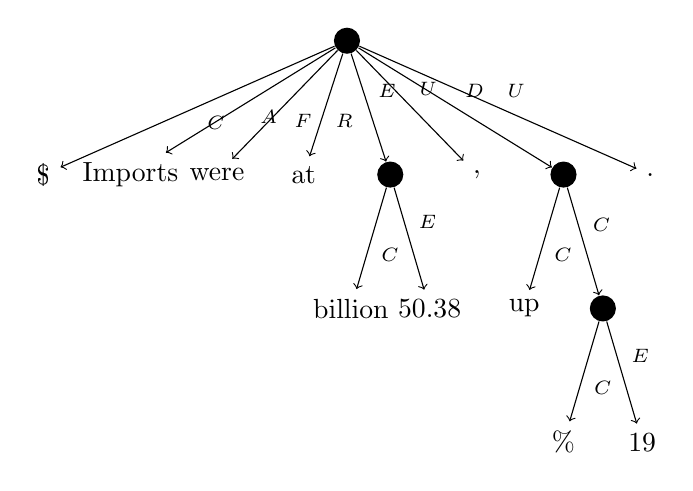
\begin{tikzpicture}[->,level distance=17mm,
  level 1/.style={sibling distance=11mm},
  level 2/.style={sibling distance=1cm},
  level 3/.style={sibling distance=1cm},
  every circle node/.append style={fill=black}]
  \tikzstyle{word} = [font=\rmfamily,color=black]
  \node (1_1) [circle] {}
  {
  child {node (1_2) [word] {\$} edge from parent node[auto] {\scriptsize $C$}}
  child {node (1_3) [word] {Imports} edge from parent node[auto] {\scriptsize $A$}}
  child {node (1_4) [word] {were} edge from parent node[auto] {\scriptsize $F$}}
  child {node (1_5) [word] {at} edge from parent node[auto] {\scriptsize $R$}}
  child {node (1_6) [circle] {}
    {
    child {node (1_7) [word] {billion} edge from parent node[auto] {\scriptsize $C$}}
    child {node (1_12) [word] {50.38} edge from parent node[auto] {\scriptsize $E$}} }edge from parent node[auto] {\scriptsize $E$}}
  child {node (1_8) [word] {,} edge from parent node[auto] {\scriptsize $U$}}
  child {node (1_9) [circle] {}
    {
    child {node (1_10) [word] {up} edge from parent node[auto] {\scriptsize $C$}}
    child {node (1_13) [circle] {}
      {
      child {node (1_14) [word] {\%} edge from parent node[auto] {\scriptsize $C$}}
      child {node (1_15) [word] {19} edge from parent node[auto] {\scriptsize $E$}} }edge from parent node[auto] {\scriptsize $C$}} }edge from parent node[auto] {\scriptsize $D$}}
  child {node (1_11) [word] {.} edge from parent node[auto] {\scriptsize $U$}} }
;
\end{tikzpicture}
  }\caption{Converted from gold UD$^{++}$ to UCCA \label{fig:wsj_0010.17_converted}}
\end{subfigure}}
  
\fbox{\begin{subfigure}{0.47\textwidth}
  \centering
  \scalebox{.95}{
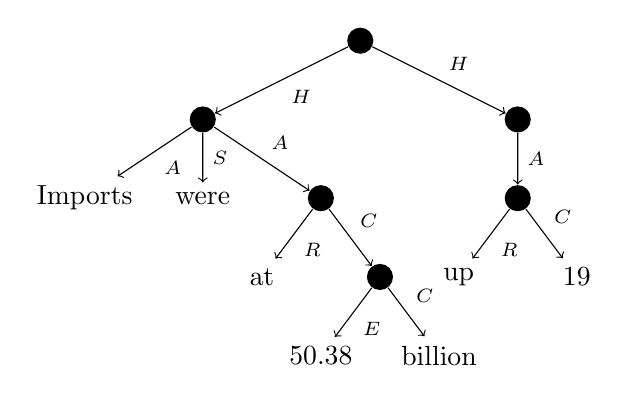
\begin{tikzpicture}[->,level distance=1cm,
  level 1/.style={sibling distance=4cm},
  level 2/.style={sibling distance=15mm},
  level 3/.style={sibling distance=15mm},
  every circle node/.append style={fill=black}]
  \tikzstyle{word} = [font=\rmfamily,color=black]
  \node (1_1) [circle] {}
  {
  child {node (1_2) [circle] {}
    {
    child {node (1_3) [word] {Imports} edge from parent node[auto] {\scriptsize $A$}}
    child {node (1_4) [word] {were} edge from parent node[auto] {\scriptsize $S$}}
    child {node (1_5) [circle] {}
      {
      child {node (1_6) [word] {at} edge from parent node[auto] {\scriptsize $R$}}
      child {node (1_7) [circle] {}
        {
        child {node (1_8) [word] {50.38} edge from parent node[auto] {\scriptsize $E$}}
        child {node (1_9) [word] {billion} edge from parent node[auto] {\scriptsize $C$}} }edge from parent node[auto] {\scriptsize $C$}} }edge from parent node[auto] {\scriptsize $A$}} }edge from parent node[auto] {\scriptsize $H$}}
  child {node (1_10) [circle] {}
    {
    child {node (1_11) [circle] {}
      {
      child {node (1_12) [word] {up} edge from parent node[auto] {\scriptsize $R$}}
      child {node (1_13) [word] {19} edge from parent node[auto] {\scriptsize $C$}} }edge from parent node[auto] {\scriptsize $A$}} }edge from parent node[auto] {\scriptsize $H$}} }
;
\end{tikzpicture}  
  }\caption{Manually annotated UCCA \label{fig:wsj_0010.17_orig}}
  
\end{subfigure}}

\caption{UCCA graphs for sentence \lstinline{wsj_0010.17}\label{fig:wsj_0010.17}}

\end{figure}

\paragraph{Conversion of automatically parsed UD annotations.}


\section{Learned label reassignment}\label{sec:learning}


\section{Experiments}\label{sec:experiments}

\begin{table*}[t]
\centering
\small
\setlength\tabcolsep{2pt}
\begin{tabular}{l|ccc|ccc||ccc|ccc||ccc|ccc}
& \multicolumn{6}{c||}{\footnotesize \bf English}
& \multicolumn{6}{c||}{\footnotesize \bf French}
& \multicolumn{6}{c}{\footnotesize \bf German} \\
\hline
& \multicolumn{3}{c|}{\footnotesize \bf {\#} tokens}
& \multicolumn{3}{c||}{\footnotesize \bf {\#} sentences}
& \multicolumn{3}{c|}{\footnotesize \bf {\#} tokens}
& \multicolumn{3}{c||}{\footnotesize \bf {\#} sentences}
& \multicolumn{3}{c|}{\footnotesize \bf {\#} tokens}
& \multicolumn{3}{c}{\footnotesize \bf {\#} sentences} \\
& \footnotesize \bf train & \footnotesize \bf dev & \footnotesize \bf test
& \footnotesize \bf train & \footnotesize \bf dev & \footnotesize \bf test
& \footnotesize \bf train & \footnotesize \bf dev & \footnotesize \bf test 
& \footnotesize \bf train & \footnotesize \bf dev & \footnotesize \bf test
& \footnotesize \bf train & \footnotesize \bf dev & \footnotesize \bf test
& \footnotesize \bf train & \footnotesize \bf dev & \footnotesize \bf test \\
\hline
Wiki & 128444 & 14676 & 15313 & 4268 & 454 & 503 &&&&&&&&&&&& \\
20K &&& 12339 &&& 506 & 10047 & 1558 & 1324 & 413 & 67 & 67 & 79894 & 10059 & 42366 & 3429 & 561 & 2164
\end{tabular}
\caption{Number of tokens and sentences in the training, development and test sets
we use for each corpus and language.\label{tab:corpora}}
\end{table*}

\paragraph{Data.}

For UCCA, we use v1.2 of the English Wikipedia corpus \cite[\textit{Wiki};][]{abend2013universal},
with the standard train/dev/test split (see Table~\ref{tab:corpora}),
and the \textit{Twenty Thousand Leagues Under the Sea} corpora
\cite[\textit{20K};][]{sulem2015conceptual},
annotated in English, French and German.\footnote{\mbox{\url{http://github.com/huji-nlp/ucca-corpora}}}
%For English and French we use 20K v1.0,
%a small parallel corpus comprising the first five chapters of the book.
%As in previous work \cite{hershcovich2017a}, we use the English part only as an out-of-domain test set.
%We train and test on the French part using the standard split,
%as well as the German corpus (v0.9),
%which is a pre-release and still contains a considerable amount of noisy annotation.

We also use 100 English sentences from Section 02 of the Penn Treebank Wall Street Journal
(PTB WSJ),
annotated by a single expert UCCA annotator \cite{hershcovich2018multitask},
and publicly available.\footnote{\url{http://github.com/danielhers/wsj}}
These sentences had already been annotated by AMR, DM and UD$^{++}$,
and we convert their annotation to the unified DAG format.

%\paragraph{Experimental setup.}
%
%
%\paragraph{Evaluation.}
%
%
%
%\section{Results}\label{sec:results}
%
%\section{Discussion}\label{sec:discussion}
%
%
%\section{Conclusion}\label{sec:conclusion}


\bibliography{references}
\bibliographystyle{acl_natbib}

\end{document}
